% MODELO CONEM 2016
\documentclass[10pt,fleqn,a4paper]{article}
\usepackage{abcm}
\usepackage{float}
\begin{document}
    
    % CABEÇALHO
    \fancypagestyle{firststyle}
	{
   		\lhead{\emph{Anais do XXII Encontro de Iniciação Científica e Pós-Graduação do ITA - XXII ENCITA / 2019
	Instituto Tecnológico de Aeronáutica, São José dos Campos, SP, Brasil, 14 de outubro de 2019}}  
	}
    \thispagestyle{firststyle}
    \vspace{-.5cm}
    \hspace{-.8cm}
    \begin{tabular}{p{\textwidth}}
    \begin{center}
    \vspace{-.6cm}
    \title{Sistema de marcação de Futebol de Robôs Soccer 3D usando aprendizado de máquina guiado por conhecimento humano}
    \end{center}
    \textbf{Isabelle Ferreira de Oliveira}\\
    \small{Instituto Tecnológico de Aeronáutica}\\
    \small{Rua H8A, 103, CTA}\\
    \small{12.228-460 - São José dos Campos/SP}\\
    \small{Bolsista PIBIC - CNPq}\\
    \small{isabelle.ferreira3000@gmail.com}\\
    \\ 
    \textbf{Edgar Toshiro Yano}\\
    \small{Instituto Tecnológico de Aeronáutica}\\
    \small{Divisão de Ciência da Computação}\\
    \small{Praça Marechal Eduardo Gomes, 50}\\
    \small{12.229-900 – São José dos Campos / SP}\\
    \small{etyano2@gmail.com}\\
    \\ 
    \textbf{Luckeciano Carvalho Melo}\\
    \small{Instituto Tecnológico de Aeronáutica}\\
    \small{LabSCA}\\
    \small{Praça Marechal Eduardo Gomes, 50}\\
    \small{12.229-900 – São José dos Campos / SP}\\
    \small{luckeciano@gmail.com}\\
%    \authors{Nome do primeiro autor, e-mail$^1$} \\
%    \authors{Nome do segundo autor, e-mail$^1$} \\
%    \authors{Nome do terceiro autor, e-mail$^2$} \\\\
%    \institution{$^1$Nome da instituição, endereço para correspondência} \\
%    \institution{$^2$Nome da instituição, endereço para correspondência} \\
%    \\
%    \authors{\textcolor[rgb]{0.98,0.00,0.00}{Mesmo  formato para outros autores e instituições, se houver.}} \\
    \\
    \abstract{\textbf{Resumo:} Devido à alta dinamicidade existente nas partidas de futebol simulado de robôs humanoide, é fundamental possuir estratégias também dinâmicas para as mais diversas situações de jogo. Nesse sentido, agregar conhecimento e percepções humanas de qual oponente está em uma posição perigosa e deveria ser marcado - para além dessas regras simples e fixas - pode ajudar a melhorar a defesa desse time em questão.
    
Após uma fase de pesquisa, foi decidido utilizar Qt, uma framework para desenvolvimento de interfaces gráficas em C++, a fim de criar um sistema de aquisição de dados de conhecimento humano sistema para marcação de oponentes. Nessa interface, o usuário pode interagir com quadros da tela da partida fornecidos periodicamente, montando o dataset de oponentes marcáveis. Esses dados adquiridos alimentaram, então, um algoritmo de aprendizado supervisionado, uma rede neural implementado em Keras, framework para desenvolvimento de redes neurais em Python, treinando, por fim, um modelo de marcação.}\\
    \keywords{\textbf{Palavras-chave:} robótica, aprendizado supervisionado, interface gráfica, Qt, Keras. }\\
    \end{tabular}
    

    \section{INTRODUÇÃO}
    A ITAndroids é uma equipe de alunos do ITA, supervisionada por um professor, que participa de diversas competições de robótica nacionais e internacionais. Uma das categorias em que a ITAndroids participa é a do robô humanoide simulado, que consiste em desenvolver um time de robôs simulados capazes de jogar futebol. Esta tarefa envolve uma série de desafios complexos que variam desde a movimentação do robô até a sua tomada de decisões.
    
    Nesse sentido de estratégia e tomada de decisões, tem-se a questão de marcação de oponentes que estejam ofensivamente perigosos durante a partida. No futebol de robôs humanóides simulados, a marcação de oponentes pode ser muito crucial em uma partida, melhorando significantemente a defesa de um time. Essa marcação consiste em implementar um algoritmo que consiga utilizar o planejamento de trajetórias do robô de forma a dificultar que oponentes em situações de vantagem façam gols. Isso traz um desafio: decidir quais são esses jogadores adversários que estão em situação mais privilegiada em um determinado instante e deveriam ser marcados por agentes aliados. 
    
    \subsection{Interface Gráfica de Aquisição de Conhecimento Humano}
    
    Grande parte do projeto se trata da ferramenta de interface gráfica que vai captar o conhecimento humano e formar o dataset da inteligência artificial. O intuito é fazer um compilado das ideias inconscientes acerca de quais oponentes deveriam ser marcados, para posteriormente automatizar o processo por meio da inteligência artificial, indo além das condições heurísticas utilizadas atualmente no time da ITAndroids. 
    
    Para resolver esse problema, então, foi feito a interface em Qt de C++. Nessa interface, o usuário pode interagir com quadros da tela da partida fornecidos periodicamente, clicando nos jogadores a serem marcados, montando, assim, o dataset de oponentes marcáveis.
    
    \subsection{Rede Neural de Classificação com Aprendizado Supervisionado}
    
    Os dados adquiridos a partir da interação do usuário - membro da ITAndroids - com a interface gráfica são intencionados a alimentar um algoritmo de classificação com aprendizado supervisionado, a fim de tentar automatizar esse processo de marcação com conhecimento humano. 
    
    Esse algoritmo foi escolhido dessa forma pela própria natureza do problema. Classifica-se cada um dos oponentes em dois tipos discretos (marcado ou não marcado), e a inteligência deve ser capaz de, para novas entradas (novas posições dos 22 jogadores e da bola, ainda sem classificação), vinculá-las a uma dessas classes pré-definidas. Isso é feito dando à inteligência acesso a informações como entradas e saídas esperadas, treinando-a como se por através de um "professor", objetivando-se encontrar a função que leva das entradas às saídas.
    
    Na implementação dessa rede neural, foi utilizado a framework Keras, em Python, e, com essa rede, foi treinado um modelo de marcação.
    
    Etapas importantes também inerentes a esse treinamento de modelo foram: pré-processamento dos dados provenientes da interface, geração de gráficos para análise das performances da rede e processamento dos resultados do algoritmo de aprendizado.

    \section{RESULTADOS OBTIDOS}
    
    Todas as ferramentas foram desenvolvidas com sucesso.
    
    \subsection{Interface Gráfica de Aquisição de Conhecimento Humano}
    
    Com o uso da plataforma Qt, foi desenvolvida esta ferramenta.
    
    Ela utiliza arquivos de texto (.txt) como entrada e gera como saída alterações nesse mesmo aquivo de texto. Esses arquivos apresentam as posições dos 22 jogadores e da bola, além de um vetor de zeros e uns (1 para oponente marcado e 0 para não marcado). A Figura \ref{fig:arquivo-de-entrada} trata-se de um desses arquivos.
    
\begin{figure}[H]
\centering
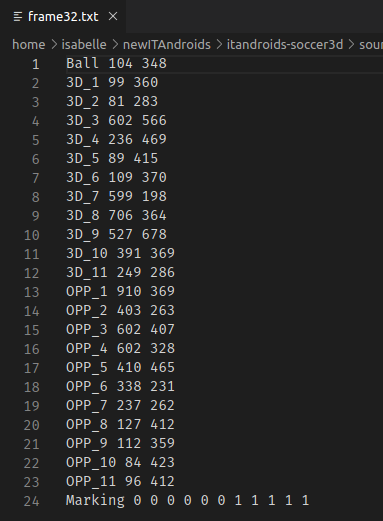
\includegraphics[width=0.4\textwidth]{figures/arquivo-de-entrada.png}
\caption{\textbf{Arquivo de entrada da interface. No exemplo, esse arquivo se trata do 32º frame analisado.}} \label{fig:arquivo-de-entrada}
\end{figure}
    
    A interação na interface se dá clicando no oponente a ser marcado, o que automaticamente altera o vetor de 0s e 1s do arquivo de entrada, além da coloração do jogador (de vermelho para verde) para fins de visualização. A ferramenta também possui quatro botões:
    
\begin{itemize}
\item prevFrame: Apresenta a visualização do frame anterior.
\item nextFrame: Apresenta a visualização do frame seguinte.
\item unmarkAll: Desmarca todos os oponentes do frame atual.
\item confirm: Atualiza o arquivo de entrada para o caso de o usuário ter desmarcado todos os oponentes.
\end{itemize}

Pode visualizar a aparência da ferramenta de interface gráfica desenvolvida na Figura \ref{fig:exemplo-interface}.

\begin{figure}
\centering
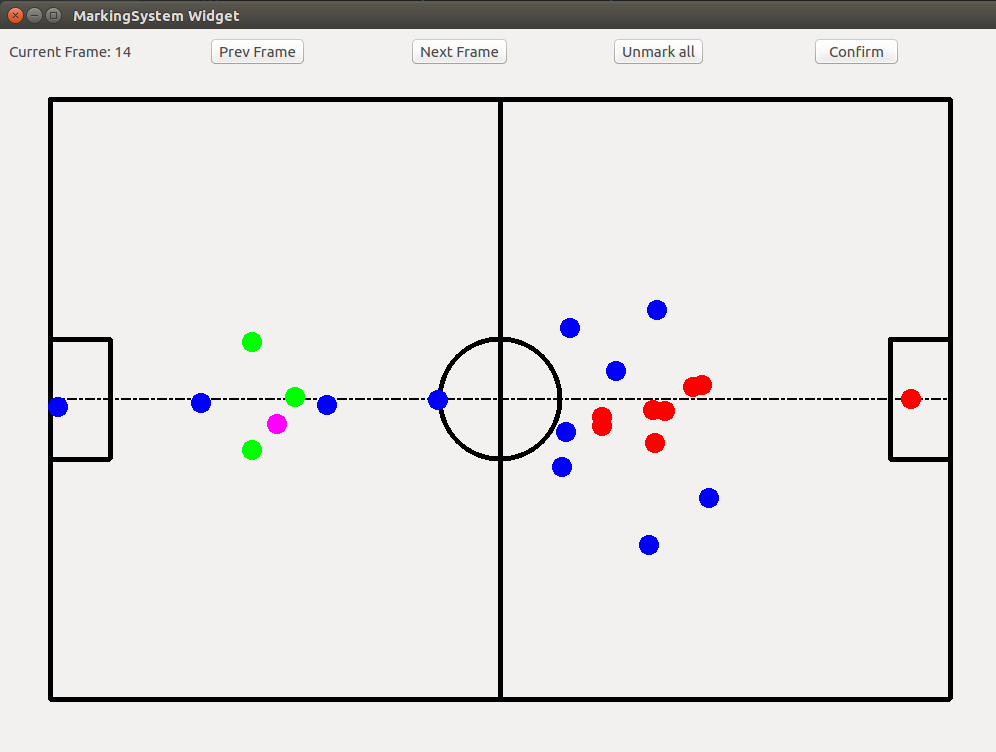
\includegraphics[width=0.6\textwidth]{figures/exemplo-interface.png}
\caption{\textbf{Aparência da ferramenta de interface gráfica, com alguns oponentes marcados. Jogadores aliados são azuis, oponentes são vermelhos e passam a ser verdes caso sejam marcados. A bola é rosa. No exemplo, esse arquivo se trata do 14º frame analisado.}} \label{fig:exemplo-interface}
\end{figure}
    
    \subsection{Rede Neural de Classificação com Aprendizado Supervisionado}
    
    O framework utilizado para escrever a rede neural foi Keras, uma biblioteca de rede neural de código aberto escrita em Python. Keras foi escolhido por ser fácil de usar, moduláveç e extensível, oferecendo um conjunto de abstrações de nível mais intuitivo, o que facilita o desenvolvimento de modelos de aprendizagem, até mesmo para deep learning \citep{whykeras}.
    
    A implementação do modelo foi feita, então, em Keras, e uma representação resumida do seu modelo foi apresentado na Figura \ref{fig:model-summary}. Esse resumo é o produzido através da chamada do método model.summary(), fornecido pela própria framework Keras. A rede consiste de 3 camadas escondidas: as duas primeiras com 64 neurônios e a última com 11 neurônios, referente as informações dos 11 jogadores oponentes (se eles devem ser marcados, ou não). A função de ativação utilizada foi a tangente hiperbólica para as duas primeiras camadas escondidas e sigmoide para a última.
    
\begin{figure}[H]
\centering
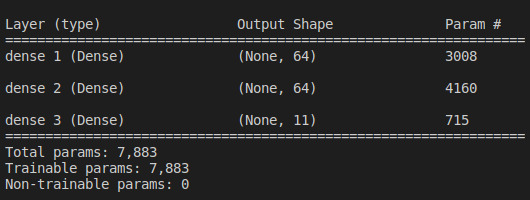
\includegraphics[width=0.5\textwidth]{figures/model-summary.jpeg}
\caption{\textbf{Resumo do modelo implentado utilizando Keras, em Python.}} \label{fig:model-summary}
\end{figure}

	Utilizou-se inicialmente um dataset de 500 frames, referentes a mais de 4 horas seguidas de partida. Esse dataset foi gerado conforme explicado anteriormente, a partir de conhecimento humano. Desse conjunto de frames, 300 (60\% do total) foram escolhidos para o treinamento da rede, 100 (20\% do total) para set de validação cruzada. Já os últimos 100 (20\% do total), foram escolhidos para o teste propriamente dito, ou seja, um dataset de entradas novas, as quais a rede jamais havia tido contato anteriormente. O treino da rede obteve um modelo com acurácia de 89.15\% no dataset de treino, 85.57\% no dataset de validação cruzada, e 86.92\% no dataset de teste.
	
	A evolução da acurácia e valor de custo com o passar das épocas foram apresentadas na Figura \ref{fig:acc-loss}. A partir dessas figuras, pode-se notar a convergência desses valores.
	
\begin{figure}[H]
	\centering
	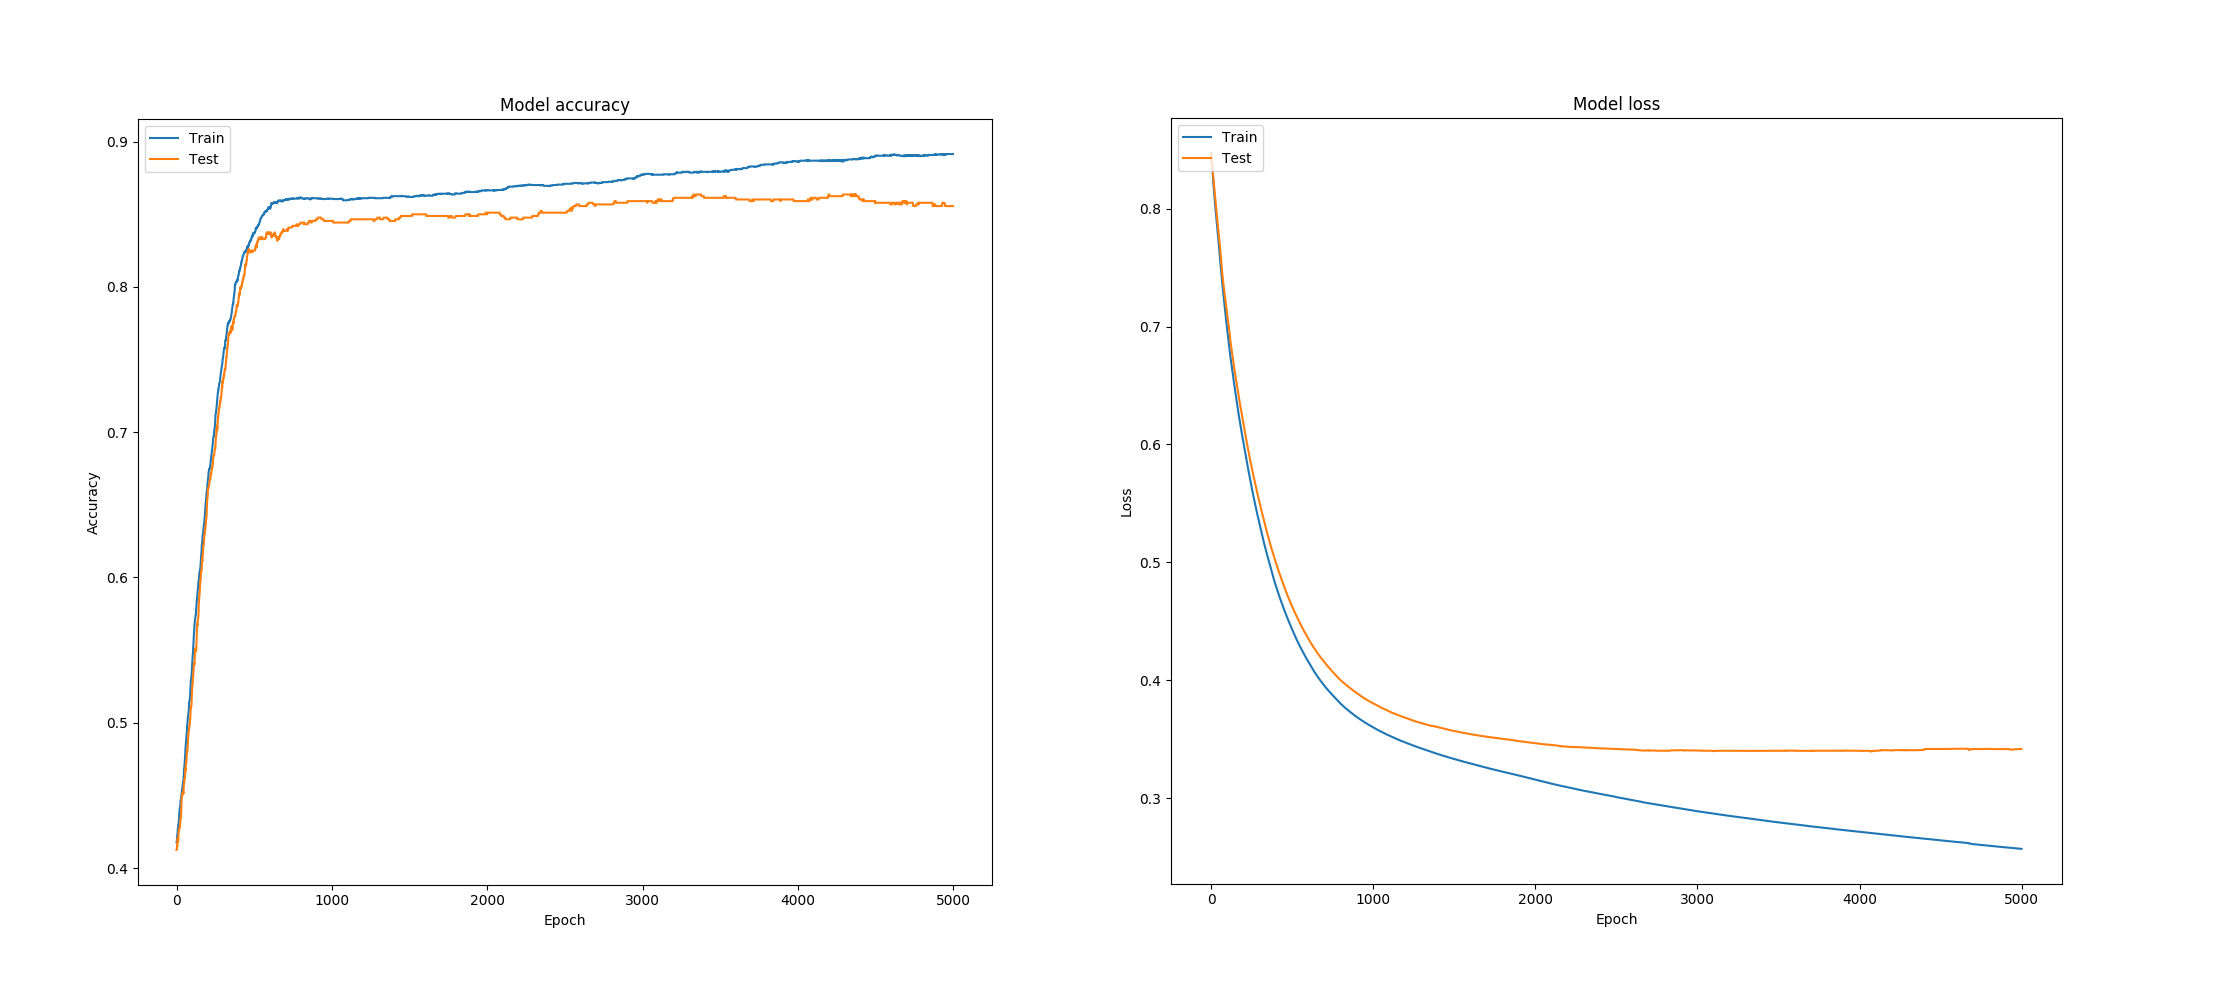
\includegraphics[width=1.0\textwidth]{figures/model-accuracy-loss.png}
   \caption{\textbf{Acurácia e função de custo, da esquerda para direita, do modelo com o passar das épocas.}} \label{fig:acc-loss}
\end{figure}
	
	Alguns exemplos dos resultados no dataset de teste foram apresentados a seguir.

	Nas Figuras \ref{fig:frame507} e \ref{fig:frame459}, consegue-se perceber um funcionamento aceitável na escolha dos oponentes a serem marcados. Nota-se também que a rede desenvolveu uma tendência de se marcar poucos oponentes, o que não necessariamente é o desejado.
	
\begin{figure}[H]
	\centering
	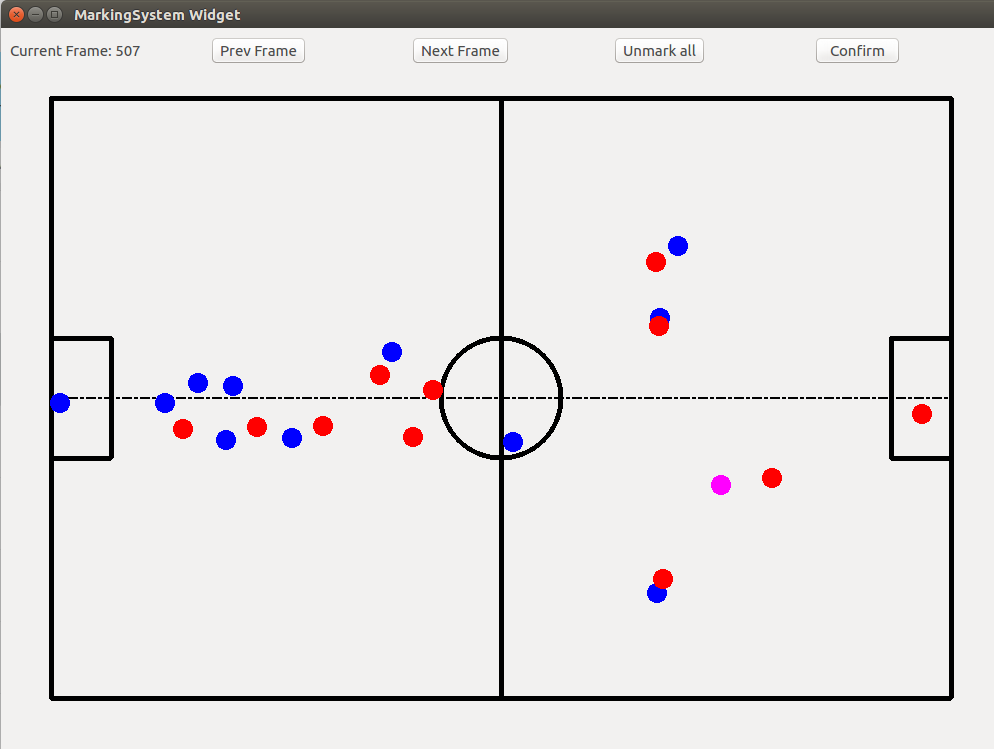
\includegraphics[width=0.6\textwidth]{figures/frame507.png}
   \caption{\textbf{Exemplo de correta marcação. Para bola presente muito à direita, no lado atacante do campo, é entendido que não se tem necessidade de marcar oponentes.}} \label{fig:frame507}
\end{figure}

\begin{figure}[H]
	\centering
	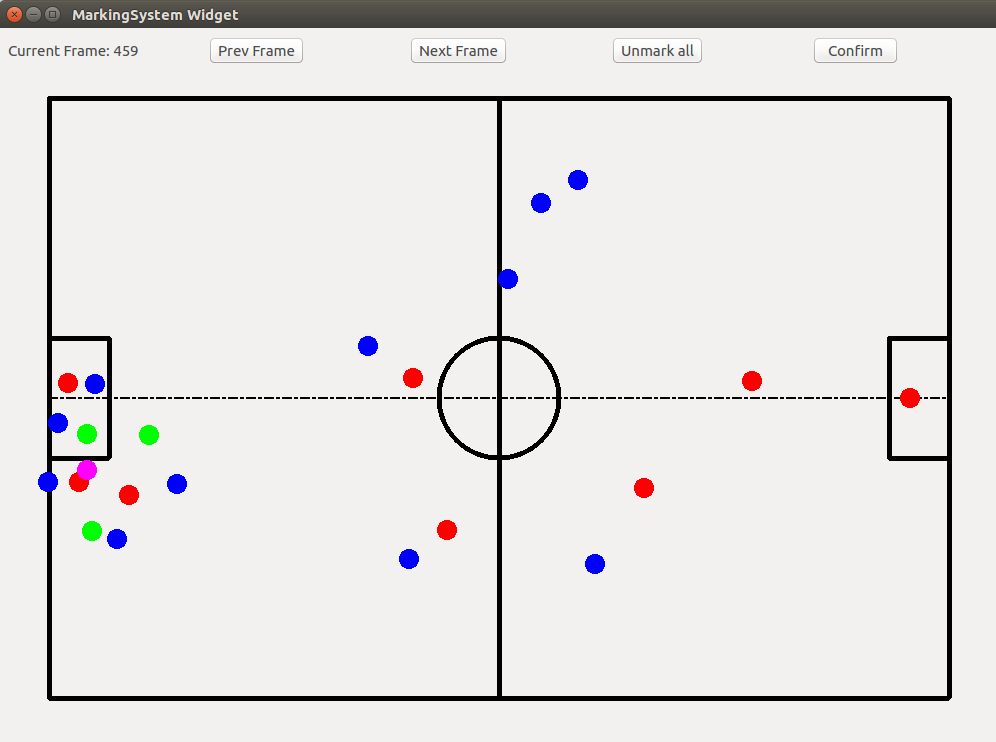
\includegraphics[width=0.6\textwidth]{figures/frame459.png}
   \caption{\textbf{Exemplo de marcação satisfatória. Nota-se a tendência da rede de marcar poucos oponentes, uma vez que há outros oponentes em situação perigosa que não estão sendo marcados.}} \label{fig:frame459}
\end{figure}

Na Figura \ref{fig:frame461}, por exemplo, pode-se perceber que essa escolha de se marcar poucos oponentes pode acabar sendo prejudicial em algumas situações reais de jogo.

\begin{figure}[H]
	\centering
	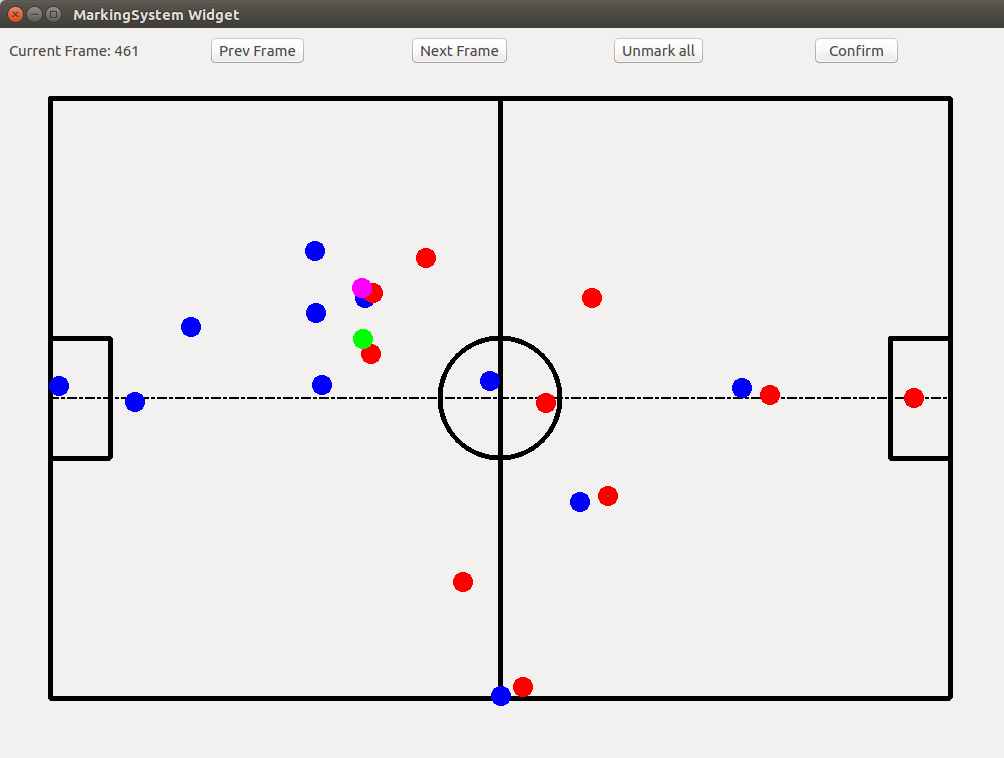
\includegraphics[width=0.6\textwidth]{figures/frame461.png}
   \caption{\textbf{Exemplo de marcação não tão satisfatória, uma vez que apenas um oponente foi marcado, bastante próximo a outro também em posição perigosa.}} \label{fig:frame461}
\end{figure}

    \subsection{Títulos e Subtítulos das Seções }

        Os títulos e subtítulos das seções devem ser digitados em fonte Times New Roman, tamanho 10, estilo negrito, e alinhados à esquerda. Os títulos das seções são com letras maiúsculas (Exemplo: \textbf{MODELO MATEMÁTICO}), enquanto os subtítulos só têm as primeiras letras maiúsculas (Exemplo: \textbf{Modelo Matemático}). Eles devem ser numerados, usando numerais arábicos separados por pontos, até o máximo de 3 subníveis. Uma linha em branco de espaçamento simples deve ser incluída acima e abaixo de cada título ou subtítulo.

    \subsection{Corpo do Texto}

        O corpo do texto é justificado e com espaçamento simples. A primeira linha de cada parágrafo tem recuo de 0,6 cm a partir da margem esquerda.

        As equações matemáticas são alinhadas à esquerda com recuo de 0,6 cm.  Elas são referidas como "Eq. (1)" no meio de uma frase, ou "Equação (1)" quando usada no início de uma sentença. Os números das equações são numerais arábicos colocados entre parênteses, e alinhados à direita, como mostrado na Eq. (1).

        Os símbolos usados nas equações devem ser definidos imediatamente antes ou depois de sua primeira ocorrência no texto. \citep{artigoMangaSBAI}

        O tamanho da fonte usado nas equações deve ser compatível com o utilizado no texto. Todos as grandezas físicas devem ter suas unidades expressas no sistema S.I. (métrico).

        \begin{equation}
        \frac{\partial^2 T}{\partial x^2} + \frac{\partial^2 T}{\partial y^2} = 0 \label{equation1}
        \end{equation}

        As tabelas devem ser centralizadas. Elas são referidas por "Tab. 1" no meio de uma frase, ou por "Tabela 1" quando usada no início de uma sentença. A legenda deve ser centralizada e localizada imediatamente acima da tabela. Anotações e valores numéricos nela incluídos devem ter tamanhos compatíveis com o da fonte usada no texto do trabalho, e todas as unidades devem ser expressas no sistema S.I. (métrico). As unidades são incluídas apenas na primeira linha ou primeira coluna de cada tabela, conforme for apropriado. As tabelas devem ser colocadas tão perto quanto possível de sua primeira citação no texto. Uma linha em branco, em espaço simples, deve ser introduzida entre a tabela, seu título e o texto.

        O estilo de borda da tabela é livre. As legendas das Figuras e das Tabelas não devem exceder 3 linhas.

        \begin{table}[ht]
            \begin{center}
                \caption{\textbf{Resultados experimentais para as propriedades de flexão dos materiais MAT1 e MAT2. Valores médios obtidos em 20 ensaios.}}
                    \begin{tabular}{|c|c|c|}
                    \hline
                    Propriedades do compósito       & CFRC-TWILL        & CFRC-4HS         \\
                    \hline
                    Resistência à Flexão  (MPa)     & 209$\pm$ 10       & 180 $\pm$  15    \\
                    \hline
                    Módulo de Flexão  (GPa)         & 57.0 $\pm$ 2.8    & 18.0 $\pm$  1.3  \\
                    \hline
                    \end{tabular}
            \end{center}
        \end{table}

        As figuras deve ser centralizadas. Elas são referenciadas por "Fig. 1" no meio de uma frase ou por "Figura 1" quando usada no início de uma sentença. Sua legenda deve ser centralizada e localizada imediatamente abaixo da figura. As anotações e numerações devem tem tamanhos compatíveis com o da fonte usada no texto, e todas as unidades devem ser expressas no sistema S.I. (métrico). As figuras devem ser colocadas o mais próximo possível de sua primeira citação no texto. Deve ser deixada uma linha em branco, de espaçamento simples, entre as figuras e o texto.
    
        \begin{figure}[h]
            \begin{center}
                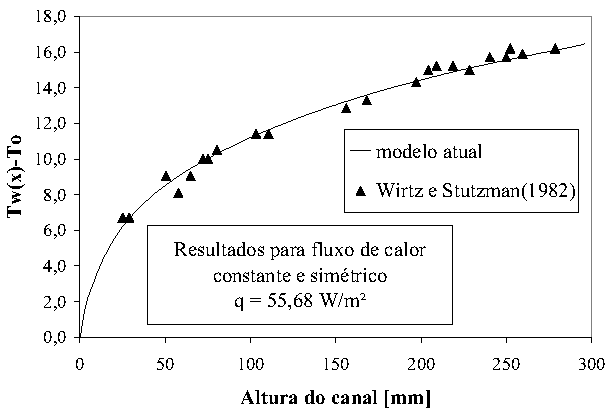
\includegraphics[angle=0, scale=.8]{figura.pdf}
            \end{center}
            \caption{\textbf{Comparação entre os resultados do presente modelo com os resultados experimentais de Wirtz e Stutzman (1982).}}
        \end{figure}

        Figuras coloridas e fotografias de alta qualidade podem ser incluídas no trabalho. Para reduzir o tamanho do arquivo e preservar a resolução gráfica, os arquivos das imagens devem ser convertidos para o  formato GIFF (para figuras com até 16 cores) ou para o formato JPEG (alta densidade de cores), antes de serem inseridos no trabalho.

        A citação das referências no corpo do texto pode ser feita nos formatos: "\citet{Bordalo89} mostra que o corpo...", ou: "Vários trabalhos (\citeauthor{Coimbra78}, \citeyear{Coimbra78}; \citeauthor{Clark86}, \citeyear{Clark86} e \citeauthor{Sparrow80},  \citeyear{Sparrow80}) mostram que a rigidez...".

        
         %   \citet{key} ==>>                Jones et al. (1990)
         %   \citet*{key} ==>>               Jones, Baker, and Smith (1990)
         %   \citep{key} ==>>                (Jones et al., 1990)
         %   \citep*{key} ==>>               (Jones, Baker, and Smith, 1990)
         %   \citep[chap. 2]{key} ==>>       (Jones et al., 1990, chap. 2)
         %   \citep[e.g.][]{key} ==>>        (e.g. Jones et al., 1990)
         %   \citep[e.g.][p. 32]{key} ==>>   (e.g. Jones et al., p. 32)
         %   \citeauthor{key} ==>>           Jones et al.
         %   \citeauthor*{key} ==>>          Jones, Baker, and Smith
         %   \citeyear{key} ==>>             1990
        
        Referências aceitas incluem: artigos de periódicos, dissertações, teses, artigos publicados em anais de congressos, livros, comunicações privadas e artigos submetidos e aceitos (com fonte identificada) e citações a páginas da internet.

        A lista de referências deve ser uma seção específica denominada Referências, localizada no fim do artigo.

        A primeira linha de cada referência deve ser alinhada à esquerda; todas as outras linhas têm recuo de 0,6 cm da margem esquerda. Todas as referências incluídas na lista devem aparecer como citações no texto do trabalho.

        As referências devem ser postas em ordem alfabética, usando o último nome do primeiro autor, seguida do ano da publicação. Exemplo da lista de referências é apresentado abaixo.


    \section{AGRADECIMENTOS}
    
        Se houver, esta seção deve ser colocada antes da lista de referências.


    % REFERÊNCIAS
    \section{REFERÊNCIAS}
        \bibliographystyle{abcm}
        \bibliography{bibliografia}

    \section{RESPONSABILIDADE AUTORAIS}

        Os trabalhos escritos em português ou espanhol devem incluir (após direitos autorais) título, os nomes dos autores e afiliações, o resumo e as palavras chave, traduzidos para o inglês e a declaração a seguir, devidamente adaptada para o número de autores.
    
        O(s) autor(es) é(são) o(s) único(s) responsável(is) pelo conteúdo deste trabalho.

% % RESUMO EM INGLES
%
%\noindent{
%   \\ 
%    \begin{tabular}{||p{\textwidth}}
%    \begin{center}
%    \vspace{-.6cm}
%    \title{AFTER FULL PAPER IN PORTUGUESE OR SPANISH, IT’S NECESSARY THE ABSTRACT IN ENGLISH}
%    \end{center}
%    \authors{First Author’s Name, e-mail1$^1$} \\
%    \authors{Second Author’s Name, e-mail$^2$} \\
%    \authors{Third Author’s Name, e-mail$^2$} \\\\
%    \institution{$^1$Institution and address for first author} \\
%    \institution{$^2$Institution and address for second and third authors} \\
%    \\
%    \authors{\textcolor[rgb]{0.98,0.00,0.00}{Same format for other authors and institutions, if any.}} \\
%    \\
%    \abstract{\textbf{Resumo:} The purpose of these instructions is to serve as a guide for formatting papers to be published in the Proceedings of the IX CONEM.  The abstract should describe the objectives, the methodology and the main conclusions of the paper in less than 4000 characters in a single paragraph.  It should not contain either formulae or bibliographic references. The full paper will be published in the proceedings of the event.}\\
%    \keywords{\textbf{Palavras-chave:} keyword 1, keyword 2, keyword 3 (up to 5 keywords) }\\
%    \end{tabular}
%}

\end{document}
